\documentclass[10pt,a4paper,DIV=14]{scrartcl}
\usepackage{ngerman}
\usepackage[latin1]{inputenc}
\usepackage[T1]{fontenc}
\usepackage{graphics}
\usepackage{graphicx}
\usepackage{subfigure}
\usepackage{amsmath}
\usepackage{amssymb}
\usepackage{mathcomp}
\usepackage{dsfont}
\usepackage[Algorithmus]{algorithm}
\usepackage{algorithmic}
\usepackage{url}
\usepackage[colorlinks,linkcolor=black,urlcolor=blue,citecolor=black]{hyperref}

\title{Vorlesung Multidimensionale und Multimodale Signale, SoSe 2010}
\author{Sebastian Rockel (6095961)\\Vitali Amann (5788408)}
\date{\today}

\begin{document}
\maketitle
%Loesung zum Uebungsblatt 1:
%\section*{1 �bung (Abgabe: 14.04.2010, 8.30 Uhr, schriftlich)}

\subsection*{1. Beschreiben Sie anschaulich den Begriff Frequenz anhand verschiedener Beispiele.}
Die Frequenz ist die H�ufigkeit eines sich regelm��ig wiederholenden Vorgangs. [wikipedia]\\
Frequenzen treten in unserer (Um-)Welt �berall auf. Beispielsweise hat der Strom aus unserer Steckdose eine Frequenz von 50 Herz, er schwingt also 50 mal in der Sekunde. Eine Schwingung fasst dabei den Vorgang zusammen, in dem die schwingende Gr��e wieder am Ausgangspunkt angelangt ist. Weitere sind z.B. Puls, Bildschirmwiederholfrequenz, Lichtspektrum, Schwingfrequenz von Atomen/Teilchen.\\
Jeder K�rper scheint eine Eigenfrequenz zu haben, in der er ``schwingtn''.

\subsection*{2. Sehen Sie einen Zusammenhang zwischen dem Begriff Frequenz und der folgenden Abbildung?}
Bilder kann man neben der ikonischen Ebene auch in der spektralen Ebene betrachten. Dabei sind hohe Frequenzen f�r die scharfen Anteile und niedrige f�r die verschwommenen zust�ndig. Entsprechend kann man ein Bild mittels Hochpass sch�rfen (tiefe Frequenzen werden gefiltert) und mittels Tiefpass weich zeichnen (hohe Frequenzen werden gesperrt).\\
Das Bild enth�lt hohe und tiefe Frequenzen von 2 urspr�nglich verschiedenen Bildern. Die scharfen Anteile geh�ren zu Albert Einstein, die unscharfen Marilyn Monroe.

\subsection*{3. Lesen Sie den Artikel auf der Seite XY und vergleichen Sie dies mit der obigen Abbildung.}
Die scharfen Gesichtskonturen der Mona Lisa zeigen kein L�cheln (bzw. wenig), die Unscharfen (Schatten der Gesichtspartien, bes. Wangen) zeigen eins.\\
Das menschliche Sehsystem kann scharfe Kanten im Fokus-Zentrum sehr gut erkennen, im �u�eren Sichtfeld werden dagegen nur unscharfe Objekte wahrgenommen.\\
Sieht man nun direkt auf den Mund �berwiegt dieser in der Wahrnehmung (nicht l�chelnd). Nimmt man dagegen das Gesicht im peripheren Sichtbereich war, �berwiegen die unscharfen Konturen (l�chelnd).

%Loesung zum Uebungsblatt 2:
%\section*{2 �bung (Abgabe: 22.04.2010, 8.30 Uhr, schriftlich)}

\subsection*{1. Gegeben sei eine periodische Funktion �ber die Zeit, wie lauten die Fourierkoeffizienten?}
a) $f(t) = \sin(t)~\text{f�r}~t \in (-\pi, \pi)$\\
$a_0 = 0; ~ a_k = 0; ~ b_k = 1; ~ k = 1$\\\\
b) $f(t) = \cos(t)~\text{f�r}~t \in (-\pi, \pi)$\\
$a_0 = 0; ~ a_k = 1; ~ b_k = 0; ~ k = 1$\\\\
c) $f(t) = \cos(2t)~\text{f�r}~t \in (-\pi, \pi)$\\
$a_0 = 0; ~ a_k = 1; ~ b_k = 0; ~ k = 2$\\\\
d) $f(t) = 1~\text{f�r}~t \in (-\pi, \pi)$\\
$a_0 = 2; ~ a_k = 0; ~ b_k = 0; ~ k = (beliebig)$

\subsection*{2. Gegeben seien die Fourierkoeffizienten einer Funktion �ber die Zeit. Wie lautet die Funktion?}

\subsection*{3. Welche der Funktionen entspricht den Dirichletschen Bedingungen im Intervall $(-\pi,\pi)$}
a) $f(t) = sgn(t)$\\
Diese Funktion erf�llt nicht die Dirichletschen Bedingungen, da die Regel \textit{ii} verletzt werden. Es existieren keine links- oder rechtsseitigen Grenzwerte in den Punkt $t = 0$.\\\\
b) $f(t) = 1~\text{falls}~t \in \mathds{Z}~\text{, sonst}~f(t) = 0$\\
Diese Funktion erf�llt nicht die Dirichletschen Bedingungen, da die Regel \textit{i} verletzt wird. Die Funktion stellt einzelne Punkte dar, die weder stetig noch monoton sind.\\\\
c) $f(t) = 1~\text{falls}~t \in \mathds{Q}~\text{, sonst}~f(t) = 0$\\
Diese Funktion erf�llt nicht die Dirichletschen Bedingungen, da die Regel \textit{i} verletzt wird. Die Funktion stellt einzelne Punkte dar, die weder stetig noch monoton sind.\\\\
d) $f(t) = \frac{1}{t}$\\
Diese Funktion erf�llt die Dirichletschen Bedingungen. Die Funktion l�sst sich in zwei Teilintervalle aufteilen, die stetig und monoton sind und f�r den Punkt $t_0 = 0$ gilt die Regel \textit{ii}, f�r die Funktion $f(t)$ existieren der links- und rechtsseitigen Grenzwert.\\\\
e) $f(t) = \cos(\frac{1}{t})$\\
Diese Funktion erf�llt nicht die Dirichletschen Bedingungen, da die Regel \textit{i} verletzt wird. Die Funktion kann zwar in Intervalle aufgeteilt werden, die stetig und monoton sind, allerdings ist die Anzahl dieser Intervalle unendlich.\\\\ 
f) $f(t) = t~\text{mod}~1$\\
Diese Funktion erf�llt die Dirichletschen Bedingungen. Diese Funktion liefer immer $0$ als Ergebnis. Somit erf�llt sie beide Bedingungen.

%Loesung zum Uebungsblatt 3:
%\section*{3. \"Ubung (Abgabe: 28.04.2010, 8.30 Uhr, schriftlich)}

\subsection*{1. Berechnen Sie $z_{1}+z_{2}, z_{1}-z_{2}, z_{2}-z_{1}, z_{1}\cdot z_{2}, z_{1}/z_{2}, z_{1}^{*}\cdot z_{2}, z_{1}/z_{2}^{*}$ f\"ur}
c) $z_{1}=4-5j, z_{2}=4+5j$

\subsection*{2. Gegeben sei eine periodische Funktion \"uber die Zeit, wie lauten die Koeffizienten der \emph{komplexen} Fourierreihe?}
a) $f(t) = \sin(t)~\text{f\"ur}~t \in (-\pi, \pi)$\\
$a_0 = 0; ~ c_{1} = -\frac{1}{2}j; ~ \bar{c_{1}} = \frac{1}{2}j;$\\\\
b) $f(t) = \cos(t)~\text{f\"ur}~t \in (-\pi, \pi)$\\
$a_0 = 0; ~ c_{1} = \frac{1}{2} = \bar{c_{1}};$\\\\
c) $f(t) = \cos(2t)~\text{f\"ur}~t \in (-\pi, \pi)$\\
$a_0 = 0; ~ c_{2} = \frac{1}{2} = \bar{c_{2}};$\\\\
d) $f(t) = 1~\text{f\"ur}~t \in (-\pi, \pi)$\\
$a_0 = 2; ~ c_{k} = 0 = \bar{c_{k}};$\\\\
e)$f(t)=sin(t)+cos(t)~\text{f\"ur}~t \in (-\pi, \pi)$\\
$a_0 = 0; ~ c_{1} = \frac{1}{2}(1-j); ~ \bar{c_{1}} = \frac{1}{2}(1+j);$\\\\

\subsection*{3. Gegeben seien die Fourierkoeffizienten einer Funktion \"uber die Zeit. Wie lautet die Funktion?}
Siehe Abbildungen \ref{fig:3.3.a},  \ref{fig:3.3.b}.
\begin{figure}[p] %  figure placement: here, top, bottom, or page
   \centering
   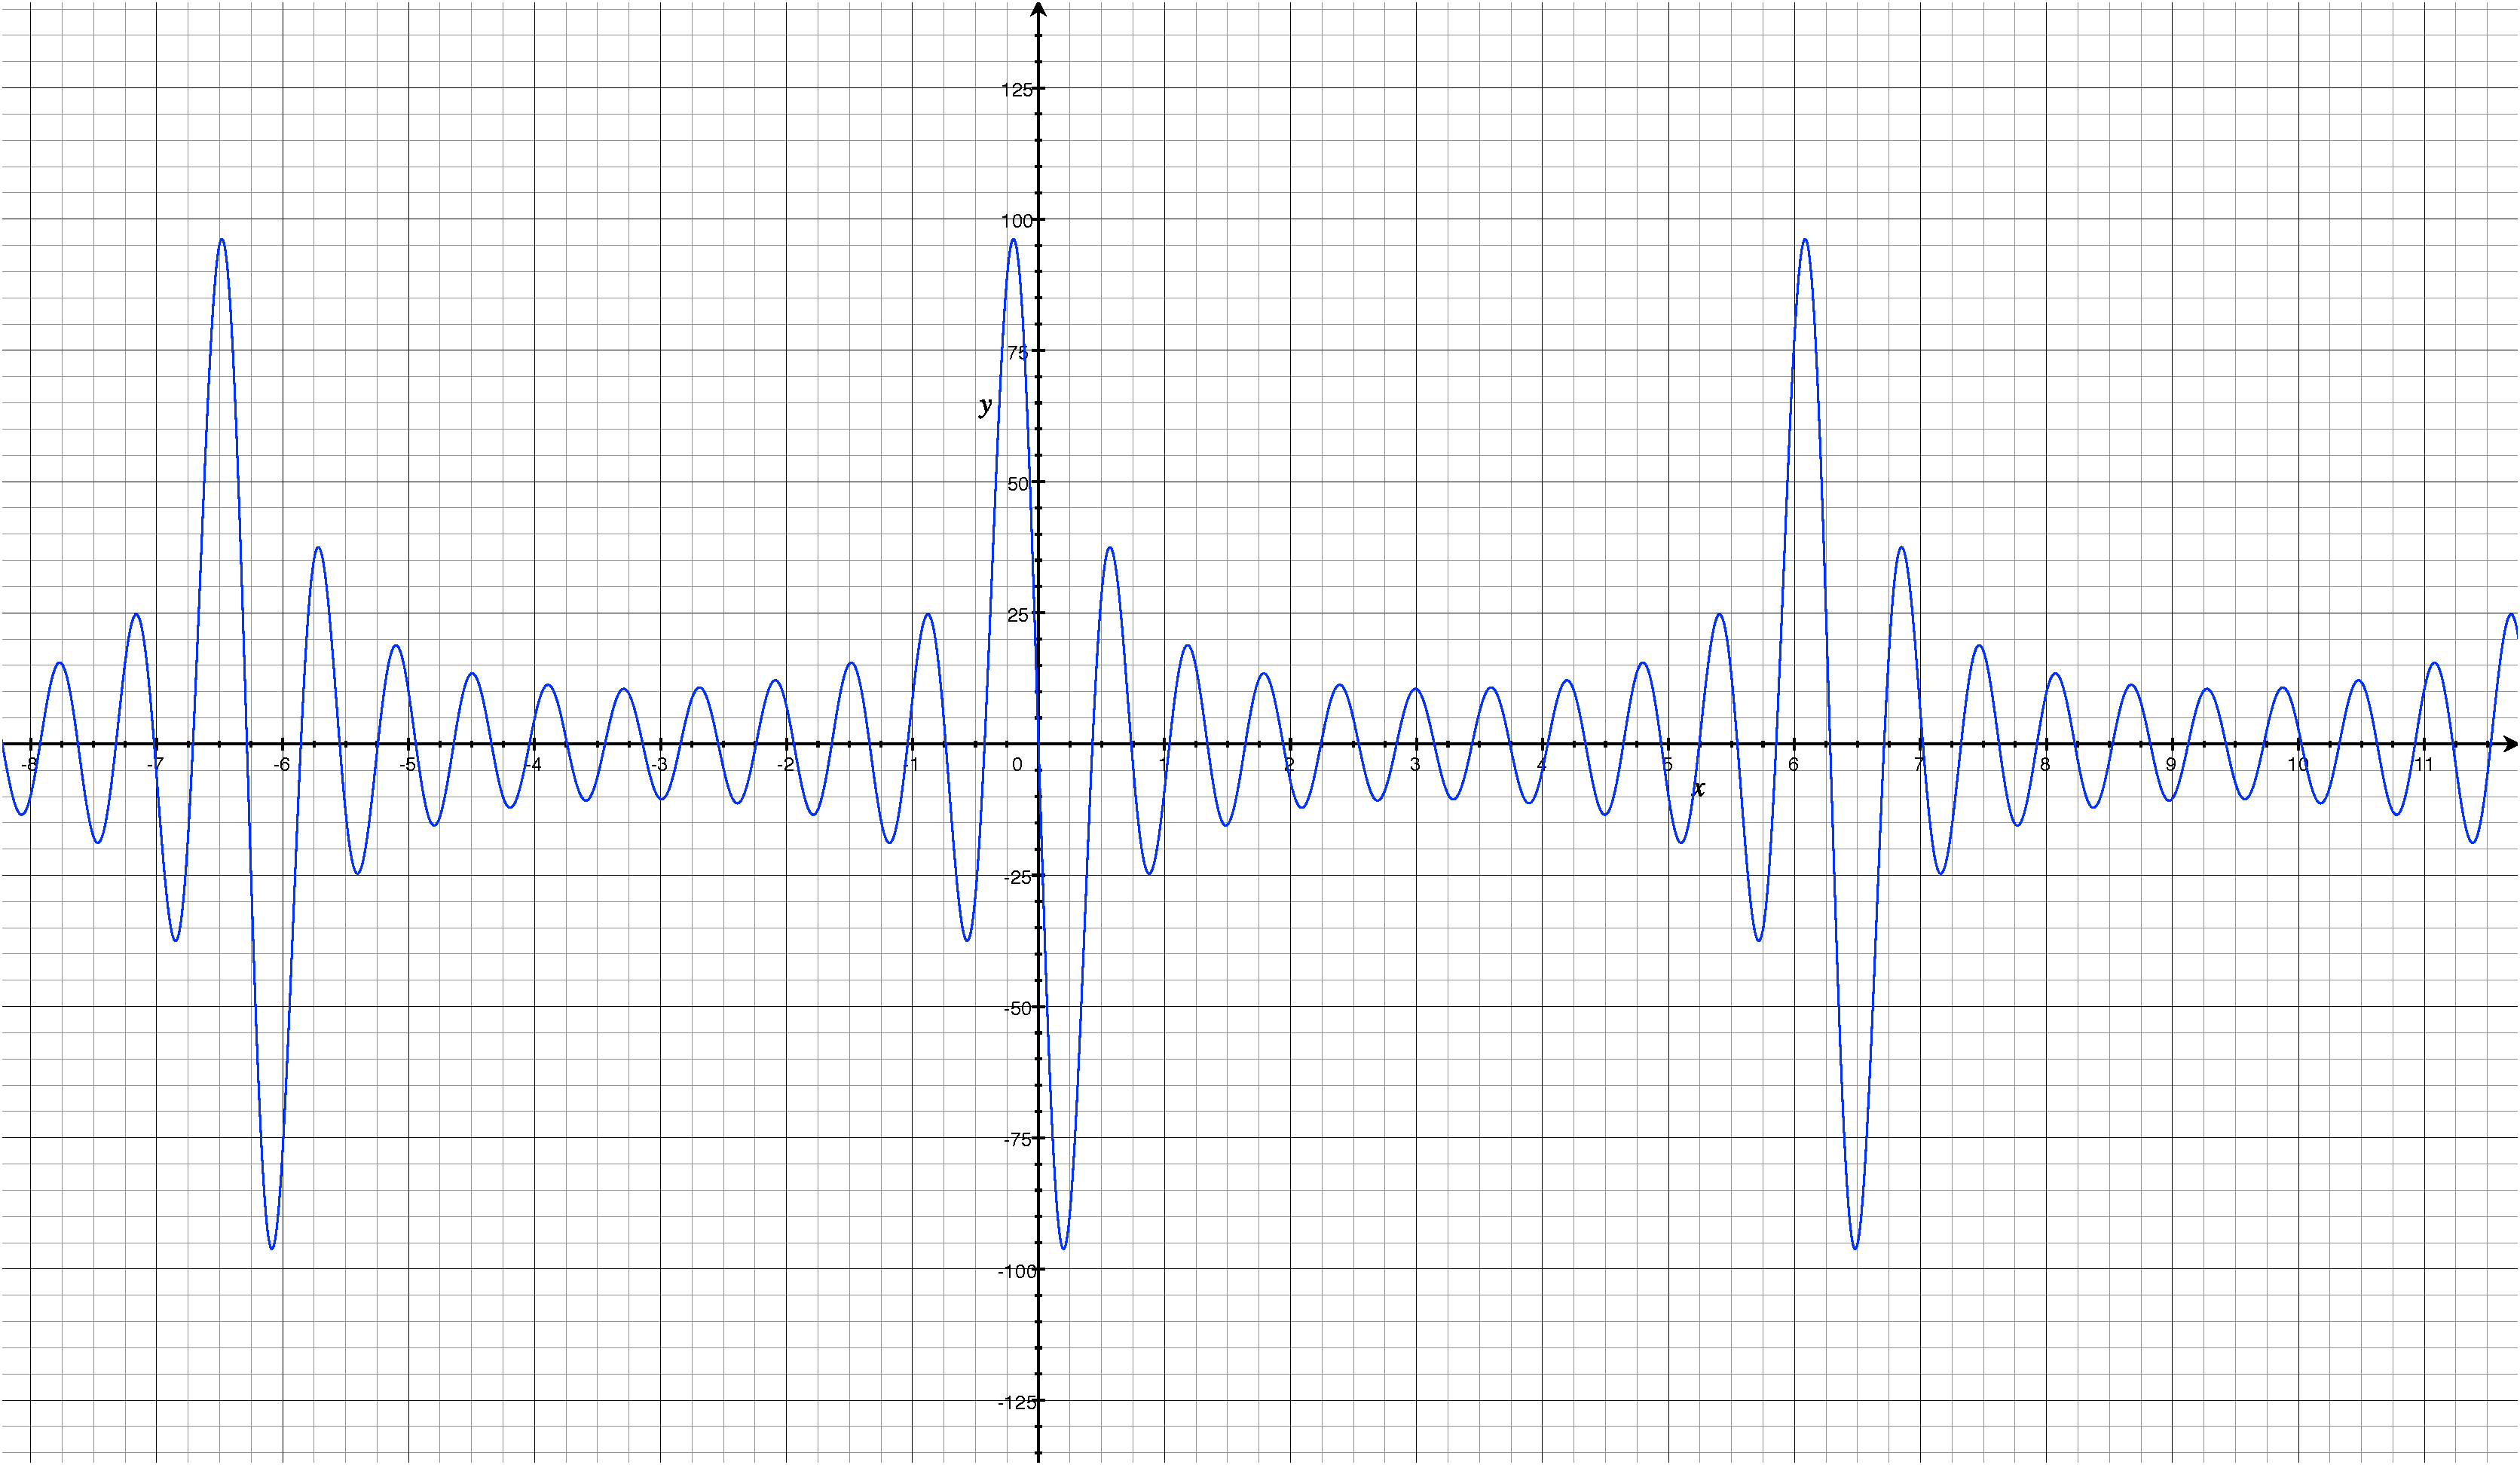
\includegraphics[width=1.0\textwidth]{Uebung3/Aufgabe_3_3_a_1.pdf} 
   \caption{$s(t)=\sum_{k=1}^n b_{k}sin(kt)=\sum_{k=1}^{n} jke^{jkt}-jke^{-jkt}, b_{k=-2k}, n=10$}
   \label{fig:3.3.a}
\end{figure}
\begin{figure}[p] %  figure placement: here, top, bottom, or page
   \centering
   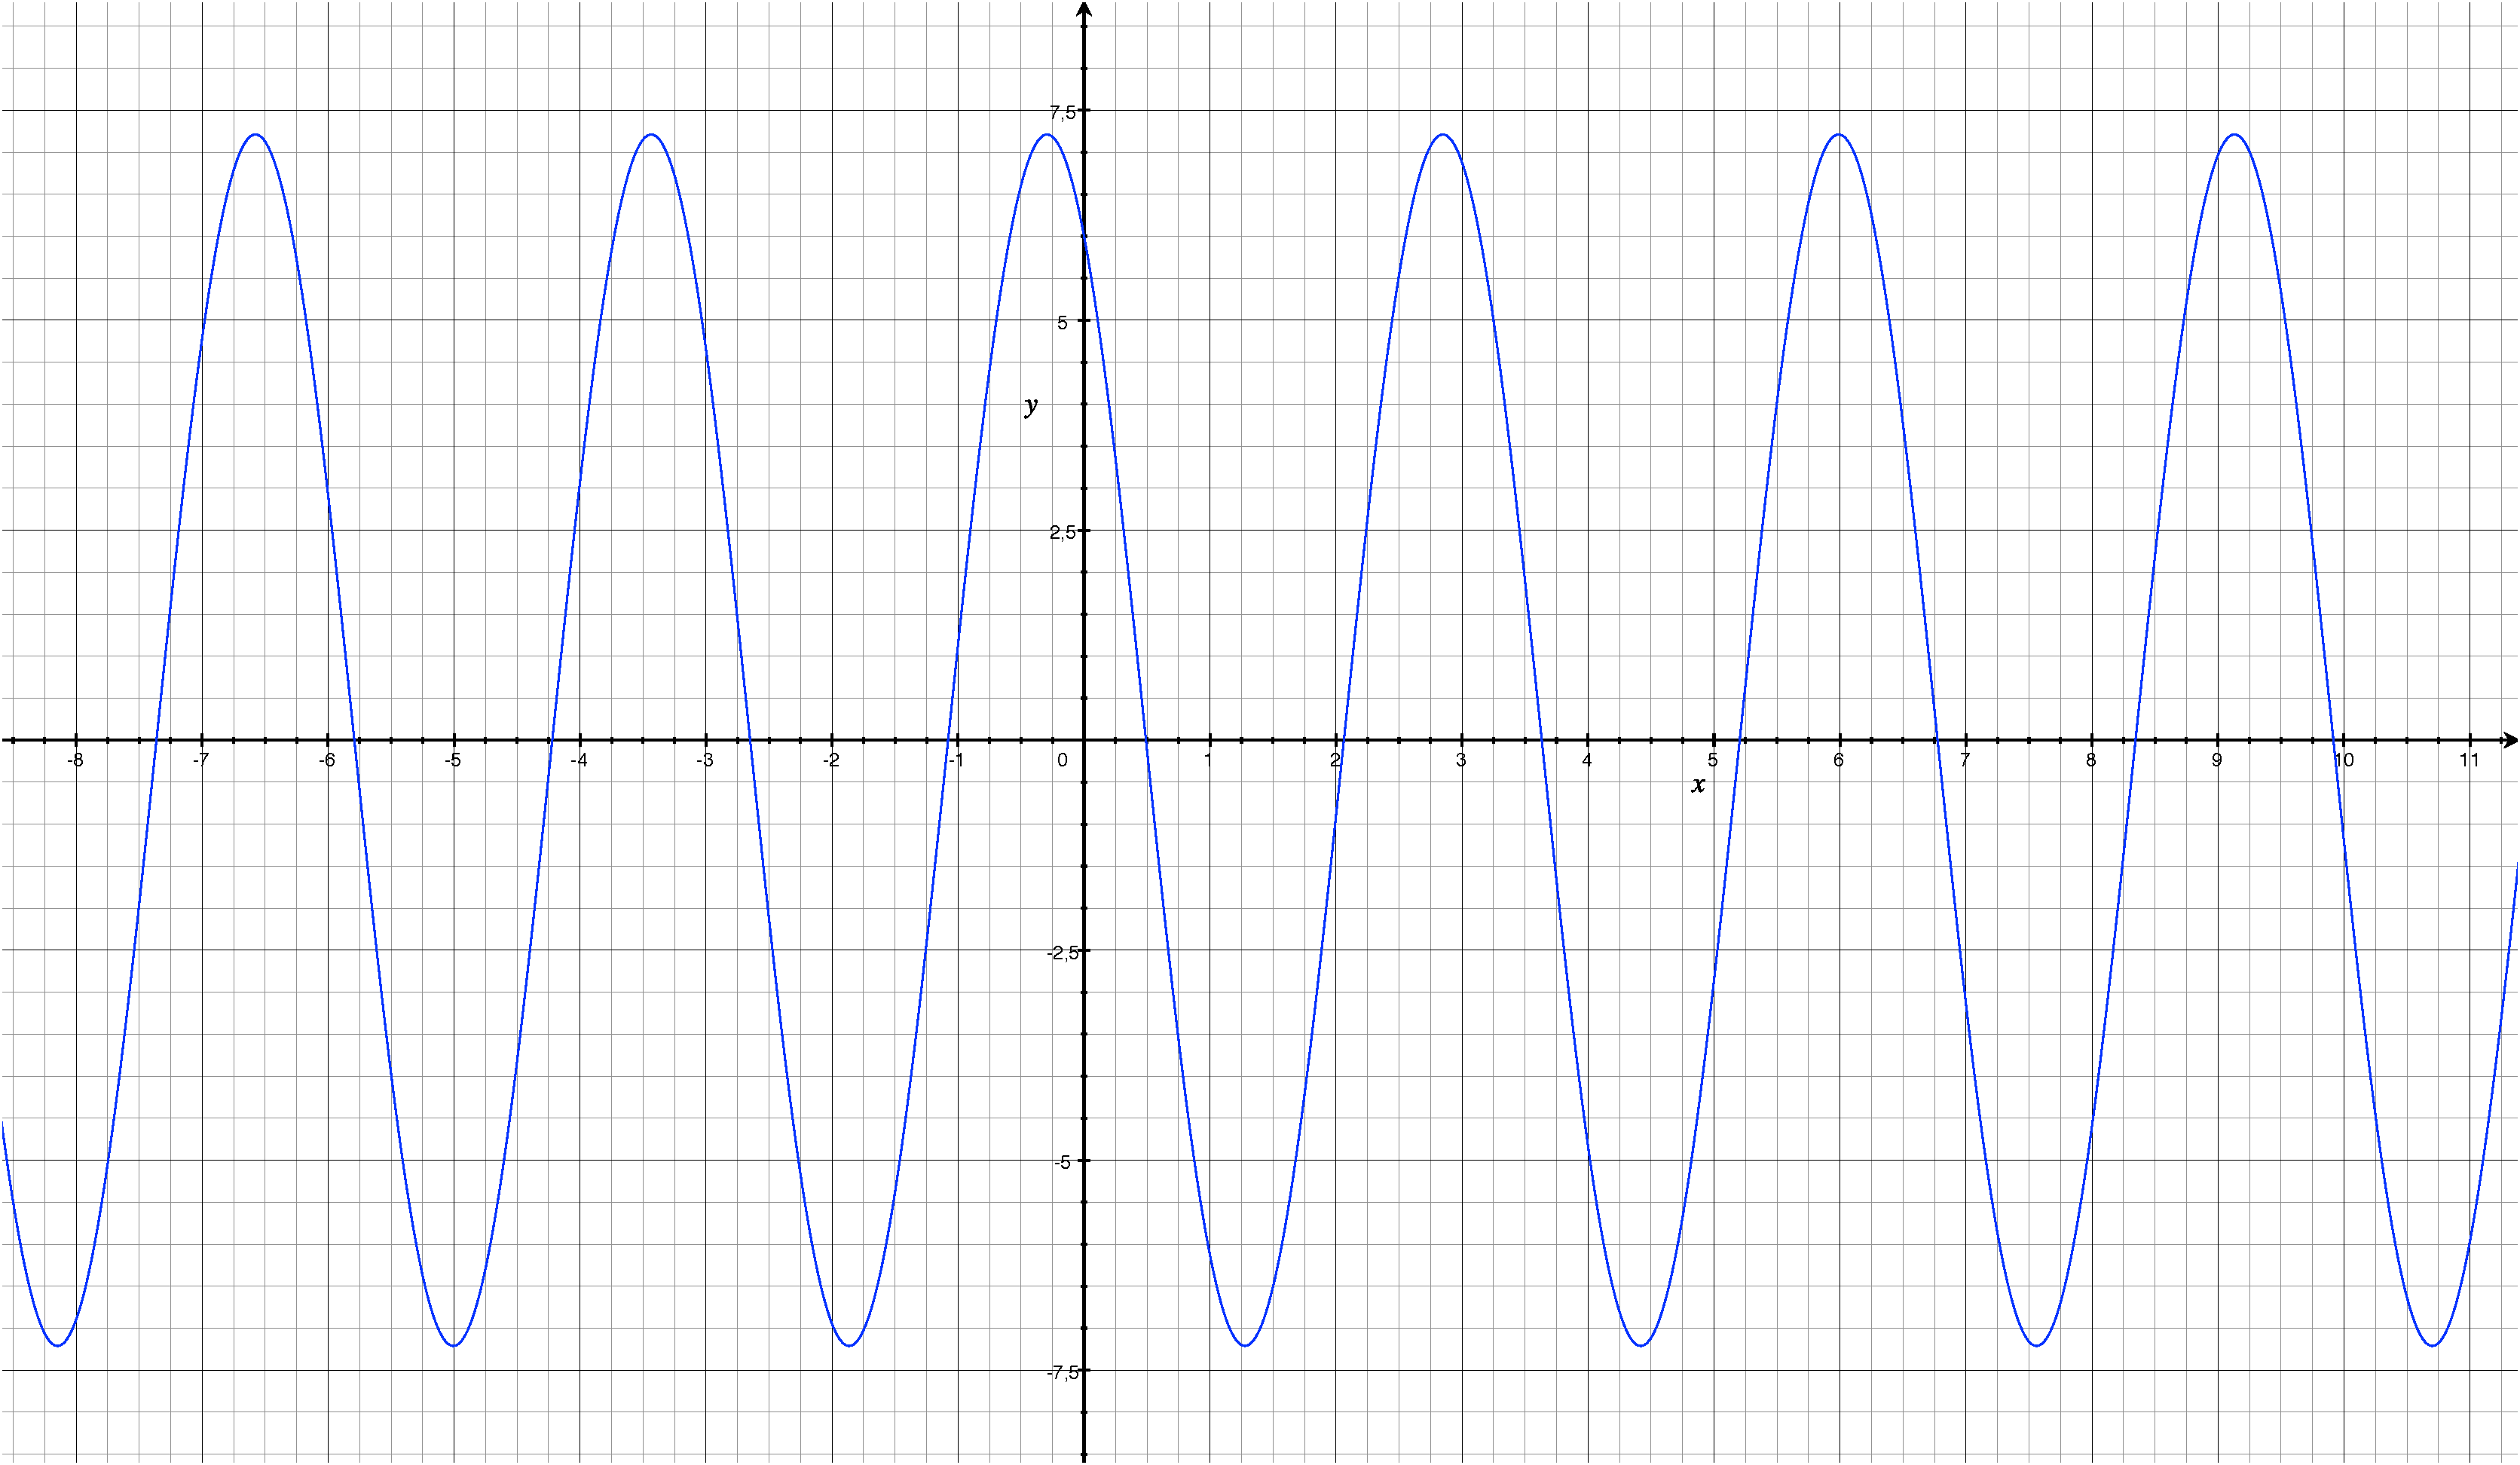
\includegraphics[width=1.0\textwidth]{Uebung3/Aufgabe_3_3_b.pdf} 
   \caption{$s(t)= 6cos(2t)-4sin(2t)=(3+2j)e^{j2t}+(3-2j)e^{-j2t}$}
   \label{fig:3.3.b}
\end{figure}

%Loesung zum Uebungsblatt 5:
%\section*{5. \"Ubung (Abgabe: 02.06.2010, 8.30 Uhr, schriftlich)}

\subsection*{1. Leiten Sie die Fouriertransformierte der Funktion $\delta_{x}(x,y):=\delta(x)$ her, wobei $\delta(x)$ die eindimensionale Dirac-Sto{\ss}-Funktion bezeichnet.}
%Siehe Abbildung \ref{fig:5.1}.
\begin{figure}[h] %  figure placement: here, top, bottom, or page
   \centering
   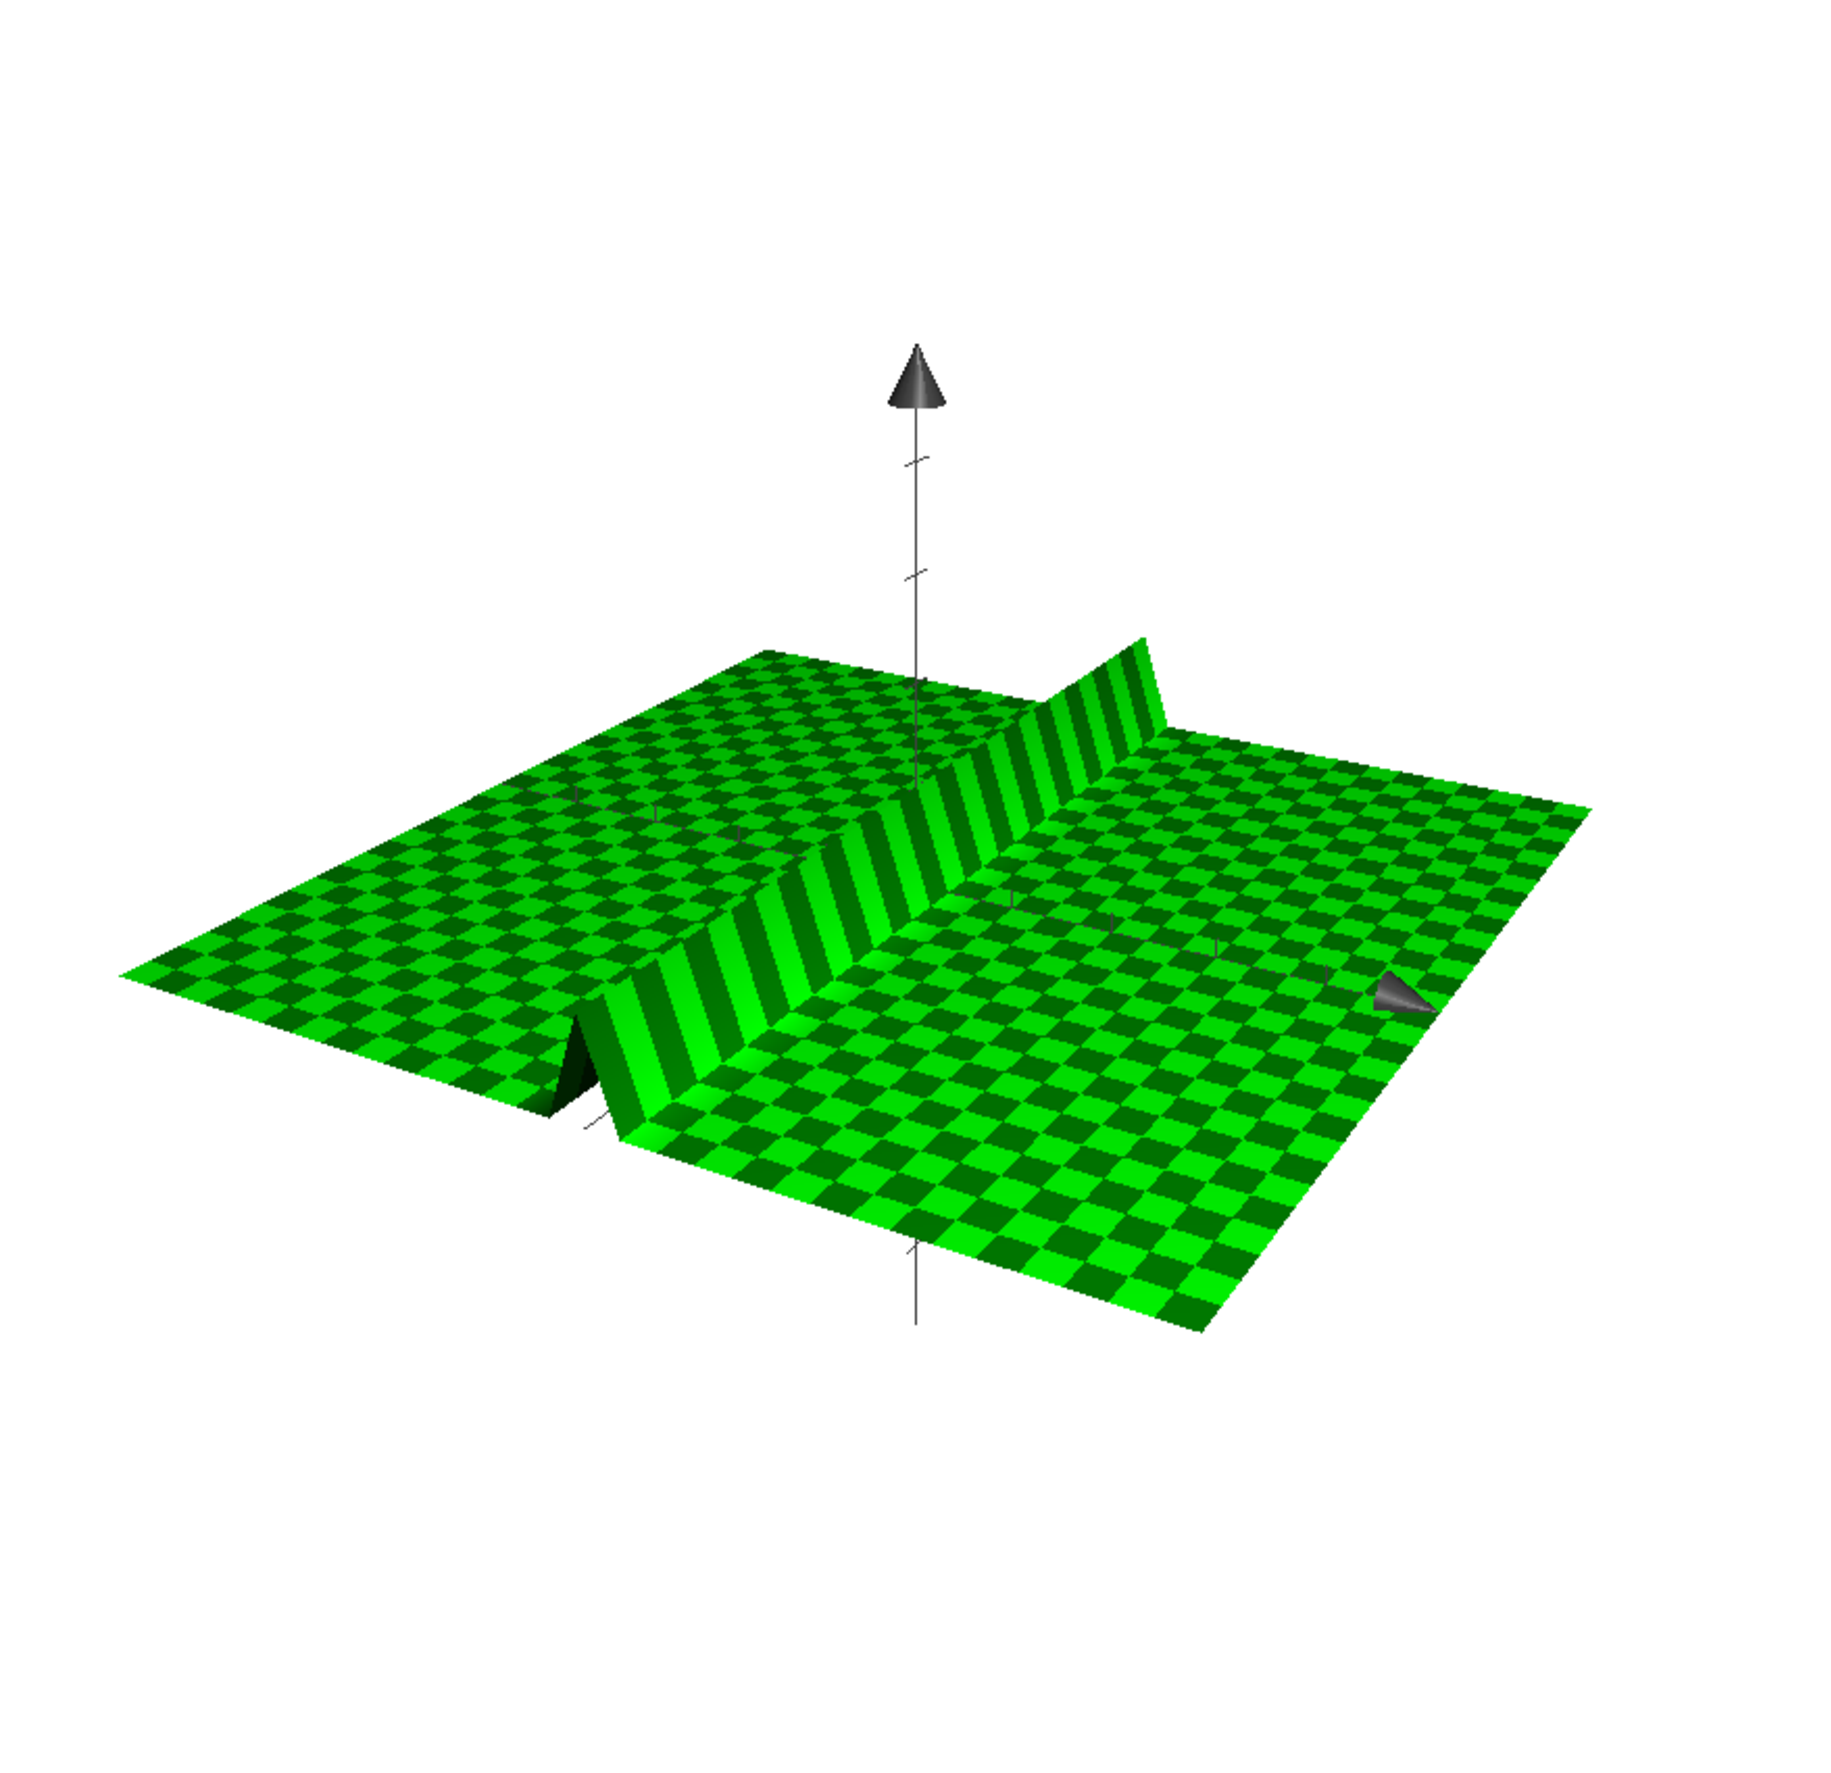
\includegraphics[width=0.8\textwidth]{Uebung5/5_1.pdf} 
   \caption{$\delta_{x}(x,y)$}
   \label{fig:5.1}
\end{figure}

\begin{eqnarray*}
f(x,y) & = & f_{x}(x)\cdot f_{y}(y) \\
\delta_{xy}(x,y) & = & \delta(x)\cdot\delta(y) \\
\delta_{x}(x,y) &=& \delta(x)\cdot 1(y) \\ \\
F(\delta(x)) &=& 1(\omega) \\ \\
F(\delta(x)\cdot 1(y)) &=& \delta(x) * 1(y) = 1(\omega) \; _{\square}
\end{eqnarray*}

\subsection*{2. Beschreiben Sie anschaulich das Ergebnis der Faltung eines zweidimensionalen Signals mit der Funktion $\delta_{x}(x,y)$. Was bedeutet dies im Frequenzbereich?}

\begin{eqnarray*}
\delta_{x}(x,y)*f(u,v) &=& \mathbf{F(\delta_{x}(x,y))}\cdot F(f(u,v)) \; \hbox{(Faltungstheorem)} \\
F(\delta_{x}(x,y)) &=& \mathbf{1(\omega)} \\
\end{eqnarray*}
\\
Im Ortsraum bedeutet die Faltung eine Ausblendung der x-Achse der zweidimensionalen Funktion. Die y-Achse bleibt erhalten (siehe Abbildung \ref{fig:5.1}). Dieses Ergebnis beruht auf der Sieb/Ausblend-Eigenschaft der $\delta$-Funktion. \\
Im Frequenzbereich bedeutet die Multiplikation mit $1(\omega)$ eine die zweidimensionale Funktion erhaltende (neutrale) Operation.

\subsection*{3. Berechnen Sie das Integral unter der Funktion $\delta^{2}(x,y):=\delta_{x}(x,y)\cdot\delta_{y}(y,x)$.}
\begin{align*}
& \int{\delta^{2}(x,y)~dx~dy}\\
= & \int{\delta_{x}(x,y)\cdot\delta_{y}(y,x)~dx~dy}\\
= & \int{\delta_{x}(x,y)~dx}~\cdot~\int{\delta_{y}(y,x)~dy}\\
= & \int{\delta(x) \cdot 1(y)~dx}~\cdot~\int{\delta(y) \cdot 1(x)~dy}\\
= & 1 \cdot 1\\
= & 1
\end{align*}

\subsection*{4. Gegeben sei eine beliebige reellwertige Bildfunktion $f(x,y)$. Nun faltet man diese Funktion mit einer geraden reellwertigen Funktion $g$ (d.h. $g(x,y)=g(-x,-y)$). Wie ver\"andert sich das Quadrat des Phasenspektrums?}
Phasenspektrum ist definiert als $\Phi = \arctan{\frac{Im(u,v)}{Re(u,v)}}$
Bei der Faltung einer beliebigen reellwertige Bildfunktion $f(x,y)$ mit einer geraden reellwertigen Funktion $g$ m\"ussen zwei F\"alle betrachtet werden:
\begin{enumerate}
\item Eine gerade reellwertige Bildfunktion $f(x,y)$ gefaltet mit $g$. Bei der Faltung entsteht wieder eine gerade reellwertige Funktion. Die Funktion besitzt nur einen reellen Anteil und keinen imagin\"aren. Daraus folgt f\"ur $\Phi^2$:\\
\begin{align*}
\Phi^2 &= (\arctan{\frac{0}{Re(u,v)}})^2\\
&= (\arctan(0))^2\\
&= 0
\end{align*}
\item Eine ungerade reellwertige Bildfunktion $f(x,y)$ gefaltet mit $g$. Bei der Faltung entsteht eine gerade reellwertige Funktion mit einem ungeraden Imagin\"aranteil. F\"ur das Phasenspektrum folgt:\\
\begin{align*}
\Phi^2 &= (\arctan{\frac{Im(u,v)}{Re(u,v)}})^2\\
&= \lim_{\frac{Im(u,v)}{Re(u,v)} \rightarrow \pm\infty} (\arctan{\frac{Im(u,v)}{Re(u,v)}})^2\\
&= \frac{\pi^2}{4}
\end{align*}
\end{enumerate}

%Loesung zum Uebungsblatt 6:
%\section*{6. \"Ubung (Abgabe: 09.06.2010, 8.30 Uhr, schriftlich)}

\subsection*{1. Diskutieren Sie die komplexwertige Gabor-Transformation und ihre Fourier-Transformierte. Welchen Bezug sehen Sie zu der Klasse der Hermitischen Funktionen?}

\subsection*{2. Gegeben sei die zweidimensionale isotrope Gauss-Funktion: $Gauss_{\sigma}(x,y)$}
\subsubsection*{Berechnen Sie die Ableitung dieser Funktion nach $\sigma$, sowie die zweite Ableitung der Funktion nach x und die zweite Ableitung nach y.}
\subsubsection*{Wie stehen diese Ableitungen in Beziehung? Beachte: Die Summe der zweiten Ableitungen nach x undy wird als \emph{Laplacian of Gaussion} bezeichnet und stellt einen \"ublichen Kantenoperator dar.}
\subsubsection*{Wie kann man den \emph{Laplacian of Gaussion} in einem Gaussian Skalenraum effizient approximieren?}


%Loesung zum Uebungsblatt 7:
%\section*{7. \"Ubung (Abgabe: 16.06.2010, 8.30 Uhr, schriftlich)}

\subsection*{1.a. Wie stark muss man ein n-dimensionales Signal gl\"atten, um die Standardabweichung des Rauschens zu halbieren?}

\begin{align*}
Gegeben:\; \sigma_{reduced\;noise}^{2} &\approx \frac{1}{(2\sqrt{\pi}\sigma_{Gauss})^{n}} \sigma_{noise}^{2} \\
Ansatz:\; \sigma_{reduced\; noise} &:= \frac{1}{2}\sigma_{noise} \\
(\frac{1}{2}\sigma_{noise})^{2} &\approx \frac{1}{(2\sqrt{\pi}\sigma_{Gauss})^{n}} \sigma_{noise}^{2} \\
\frac{1}{2}\sigma_{noise} &\approx \frac{1}{(2\sqrt{\pi}\sigma_{Gauss})^{\frac{n}{2}}} \sigma_{noise},\; \sigma_{noise}>0 \\
\frac{1}{2} &\approx \frac{1}{(2\sqrt{\pi}\sigma_{Gauss})^{\frac{n}{2}}} \\
2 &\approx (2\sqrt{\pi}\sigma_{Gauss})^{\frac{n}{2}} \\
4 &\approx (2\sqrt{\pi}\sigma_{Gauss})^{n} \\
\sqrt[n]{4} &\approx 2\sqrt{\pi}\sigma_{Gauss} \\
\sqrt[n]{4}\cdot\frac{1}{2\sqrt{\pi}} &\approx \sigma_{Gauss} \\
\end{align*}
Das bedeutet, je mehr Dimensionen das Eingangssignal hat, desto geringer muss die Gl\"attung ausfallen, um die Standardabweichung des Rauschens zu halbieren.

\begin{figure}[!h] %  figure placement: here, top, bottom, or page
   \centering
   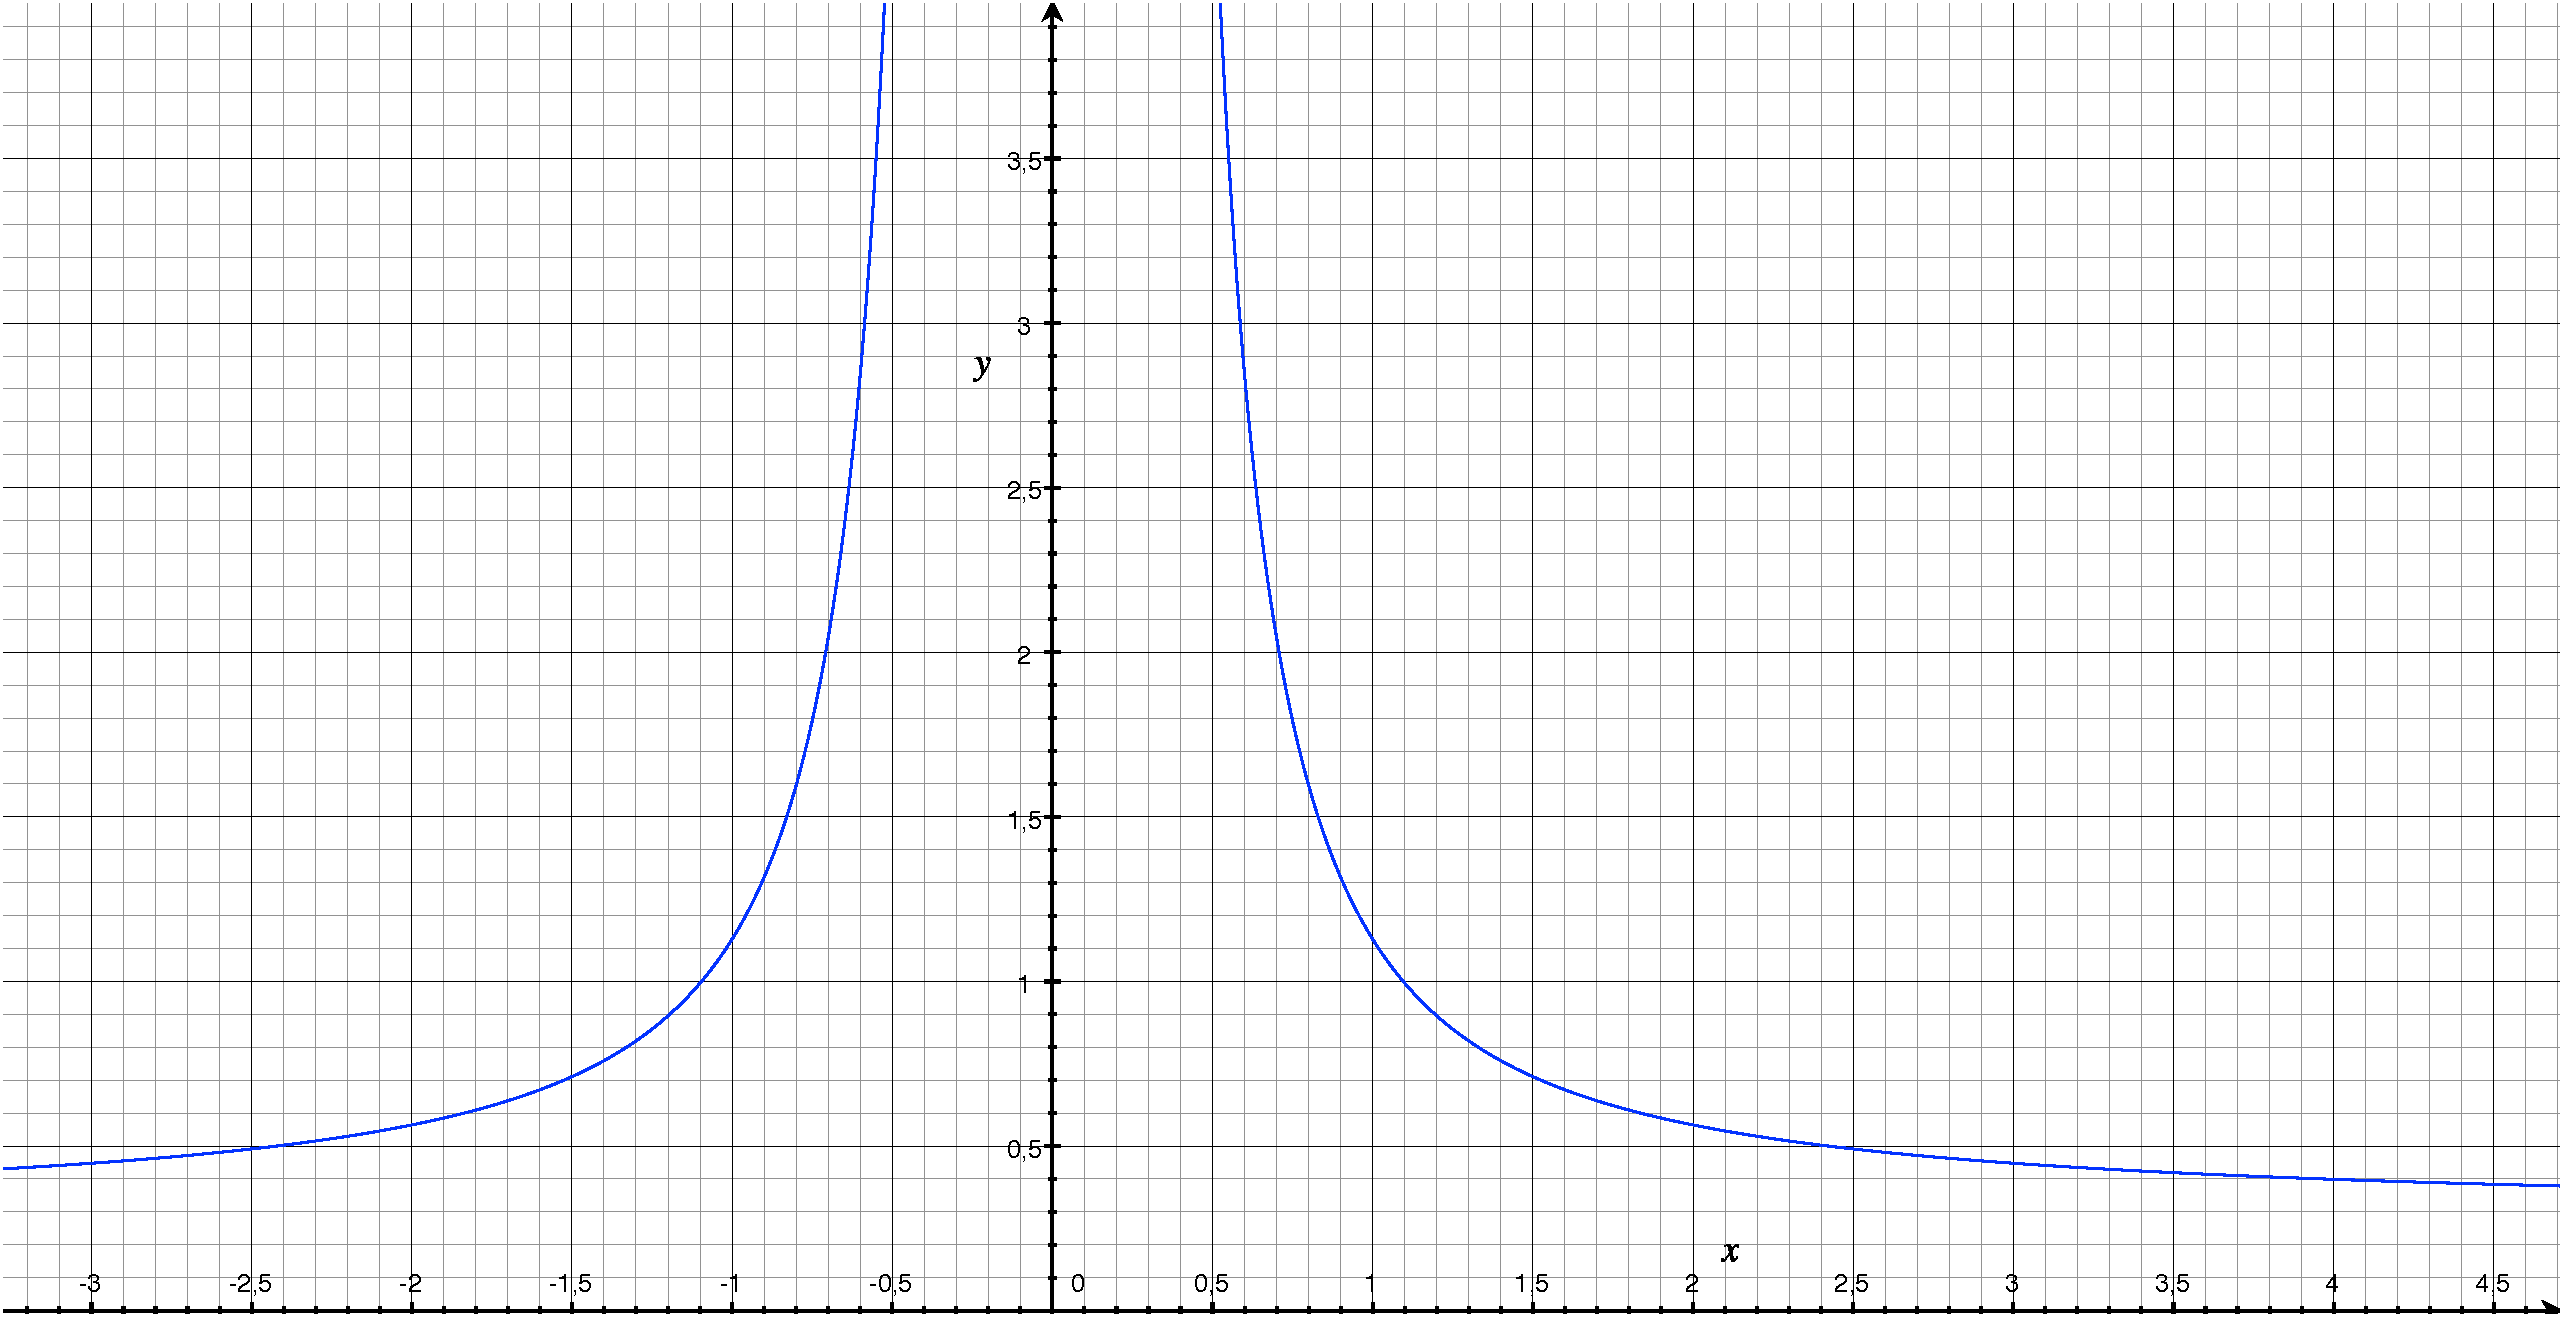
\includegraphics[height=0.17\textheight]{Uebung7/1_a.pdf} 
   \caption{Zusammenhang von Dimension (x$=\mid n \mid$) und Gl\"attung (y$=\sigma_{Gauss}$)}
   \label{fig:5.1}
\end{figure}

\subsection*{1.b. Auf welche Weise h\"angt die Varianz des Lokalisierungsfehlers f\"ur die F\"alle n=1,2,3 von dem Grad des urspr\"unglichen Rauschens und dem Grad der Gl\"attung ab? Was bedeutet das f\"ur die Anwendung von schwellenwertbasierten Kantendetektoren in verrauschten zweidimensionalen Bildern?}


%Loesung zum Uebungsblatt 8:
\section*{8. \"Ubung (Abgabe: 23.06.2010, 8.30 Uhr, schriftlich)}

\subsection*{1.Begr\"unden Sie anhand des abgebildeten Grauwertgebirges, dass das Prinzip der Kausalit\"at f\"ur einen linearen homogenen isotropen Diffusionsprozess streng genommen nicht gilt.}

Die Diffusion des abgebildeten Grauwertgebirges (und anderer Signale) entspricht einer Gl\"attung dieser (Faltung mit der Gauss-Normalverteilung im Ortsraum bzw. Zeitraum). Ferner legt man diesen Diffusionsprozess hier als linear (also unabh\"angig vom Ort im Signal), homogen (also gleichm\"a{\ss}ig \"uber dem Skalenraum) und isotrop (also lokal gleich in alle Richtungen) fest (1). \\
Nun betrachtet man die Faltung zweier Gau{\ss}-verteilungen als invariant in der Hinsicht, dass wieder eine Gau{\ss}verteilung entsteht (mit gr\"o{\ss}erem Sigma und kleinerer Amplitude). \\
Fasst man die lokalen und globalen Maxima und Sattelpunkte als lokale Gau{\ss}-verteilungen im originalem Grauwertgebirge auf, entsteht wegen (1) wieder ein Grauwertgebirge (mit kleinerer Amplitude und gr\"o{\ss}erer Bandbreite). \\
Dies l\"asst sich streng genommen beliebig oft wiederholen und man bekommt immer wieder ein, zwar sehr gegl\"attetes, aber immer noch topologisch korrektes  Signal(d.h. gleiche Anzahl Maxima/Sattelpunkte). Leider f\"uhrt die notwendige Quantisierung in der digitalen Verarbeitung zu einer stetigen Ausl\"oschung ``zu kleiner'' Extrema aufgrund der nur diskreten (Flie{\ss}komma-) Genauigkeit.

\subsection*{2. Gibt es nicht-konstante Funktionen $f: \mathbb{R}^{2} \rightarrow \mathbb{R}$, bei denen die Zahl der lokalen Maxima bei einem solchen Diffusionsprozess niemals auf 1 f\"allt?}

\subsection*{3. Wie kann man den Nachteil, dass der Gradientenbetrag an Ecken abnimmt, mit Hilfe von  Diffusionsmethoden verbessern?}
Gradientenbetrag: $\sqrt{x^{2}+y^{2}}$ \\
Idee: Gradientenbetrag nimmt an Ecken ab, da sich die zwei Richtungen (gleichstark) gegenseitig st\"oren. (aber wie?) \\
Ans\"atze:  \\
\emph{Edge-enhancing diffussion}: Diffussion entlang des Kontrastes \\
\emph{Coherence-enhancing diffusion}: Gro{\ss}e Koh\"arenz bei geriechteten (anisotropen) Strukturen

\end{document}